% DOCUMENT
%\documentclass[a4paper]{article}
\documentclass[a4paper, twocolumn]{article}

% PACKAGES
\usepackage{titlesec}
\usepackage[english]{babel}
\usepackage{blindtext}
\usepackage{graphicx} 
\usepackage{enumitem}
\usepackage{amsmath}
% \usepackage{parskip}
\usepackage{mathptmx}
% \usepackage[none]{hyphenat}
%\usepackage[showframe]{geometry}
\usepackage{layout}

% SETTINGS
% Title Format
\titleformat*{\section}{\large\MakeUppercase}
\titleformat*{\subsection}{\large\MakeUppercase}
\titleformat*{\subsubsection}{\large\bfseries}

% USER-DEFINED COMMANDS

% TITLE
\title{\Huge{Path Tracking and Obstacle Avoidance of Autonomous Mobile Robots}}
\author{Faizudeen Kajogbola} 
\date{} %BLACK DATE TO  OMIT DATE FROM TITLE

% DOCUMENT
\begin{document}%\layout

% DISPLAY TITLE
\maketitle

\setlength{\headsep}{5pt}
\setlength{\voffset}{-0.75in}   % REMOVE EXCESSIVE SPACE AT TOP OF PAGE

% INTRODUCTION
\section{Introduction}

Autonomous Mobile Robots (AMRs) are required to move around to perform some tasks, 
this makes the ability to navigate effectively and efficiently an important measure of success for any such robot.
For navigation, an AMR is required to plan a path leading to its goal point, 
generate a trajectory along the planned path, and appropriately track the generated trajectory.

Path planning involves the AMR searching for an optimal collision-free path from its initial position to some 
desired goal position which conforms to its physical constraints \cite{cai1}.
Path planning is divided into: global path planning in which the environment known completely; 
and the local path planning in which only some section of the environment is known.
Common global path planning techniques include A* heuristic search, visibility graph method, generalized Voronoi diagram, 
ant colony algorithm, genetic algorithm, and the artificial potential field method \cite{kunchev1, shi1}.

The Artificial Potential Field (APF) method draws inspiration from classical physics and was first proposed in 1986 by Khatib \cite{khatib1}.
With this method, an AMR seems to move towards its goal position and avoid obstacles instinctively. 
This is because repulsive potentials are generated to represent obstacles while attractive potentials are 
generated to represent the goal position, effectively transforming the path planning problem into an 
optimization problem \cite{ji1}.
APF gives room for the possibility of real-time online path planning. 
Globally-planned paths can be updated with local information from robot sensors- 
e.g. new location of a moving obstacle-, thereby making it possible to plan paths that avoid dynamic obstacles.
This, and its mathematical conciseness \cite{shi1} are some of the reasons why APF-based approaches 
are widely used in path planning for AMRs.
However, if special care is not taken in formulating the potential functions, the robot might get stuck at 
a local minima and never reach its goal position.
To prevent this, several methods of formulating the potential functions have been proposed. 
These include Gaussian-shaped repulsive functions \cite{koditschek1}, the super-quadratic potential function \cite{volpe1}, 
simulated annealing technique \cite{zhu1}, and methods that utilize search techniques with the capability of escaping local minima \cite{barraquand1}.

A trajectory can be generated from a planned path by time parametrization \cite{roesmann1}. 
To enable collision-free navigation, the generated trajectory must respect the dynamical and kinematical constraints of the AMR.
Due to nolinear dynamics, path tracking of AMRs is generally performed using sliding mode control \cite{yang1}, 
robust control \cite{normey-rico1}, fuzzy logic control \cite{antonelli1}, or model predictive control (MPC) \cite{ji1}.

In recent years, a lot of research efforts have been poured into implementing MPC algorithms for navigation.
Götte et al. in \cite{goette1} propose a model predictive planning and control (MPPC) approach which handles both trajectory planning and tracking.
In \cite{nolte1}, Nolte et al. present a generalized approach for path and trajectory planning with model predictive frameworks.
A contrained linear time-varying MPC was implemented by Gutjahr et al. in \cite{gutjahr1} for path tracking and trajectory optimization.
While a multiconstrained MPC was presented by Ji et al. in \cite{ji1} solely for the purpose of path-tracking.

In the following, path tracking and obstacle avoidance for an AMR is investigated.
Avoidance of static obstacles in a completely known environment is considered, while taking the robot’s kinematic limitations 
(such as its size, shape, and its steering constraints) into account.
An APF approach is used for path planning and trajectory generation, 
while a multi-constrained model predictive control is used for tracking the generated trajectory.


%===============================================================================================================%
\section{Path Planning and Trajectory Generation}
This section focuses on path planning and trajectory generation based on Artifical Potential Fields (APFs).
While many researchers have proposed a vast array of path planning techniques, APFs provide an intuitive formulation that 
allow real-time modifications of planned trajectories. A feature that becomes quite essential in a configuration space with dynamic obstacles.

The following assumptions are made in this study to simplify the mathematical representation of collision-free trajectories:
\begin{itemize}
    \item A configuration space of 50m x 50m.
    \item Static obstacles with rounded geometry and known sizes and positions.
    \item Constant longitudinal velocity of 1m/s.
\end{itemize}

\subsection{Path Planning}
Two coordinate systems are considered. The Autonomous Mobile Robot's (AMR's) body coordinate system $\mathit{o-xy}$, 
which is centered on the vehicle's center of mass with the x-axis is along the AMR's longitudinal axis, 
while the y-axis is along it's lateral axis; and a fixed earth coordinate system $\mathit{O-XY}$, 
which is defined to be colinear with the vehicle body coordinate system at the instant of path planning. 
At any point in time, the angle of rotation between both corrdinate systems is the AMR's yaw angle $\psi$. 
The position of the AMR in the fixed-earth coordinate is given as $\vec{X_{r}}$, 
the position of the goal point as $\vec{X_{g}}$ and position of obstacles as $\vec{X_{o}}$.

The universal potential ($U$) which guides the AMR to it's goal position is composed of the attractive potential ($U_{A}$) 
and the repulsive potential ($U_{R}$).

The attractive potential ($U_{A}$) is formulated such that it's minumum point is at the goal position, 
a mathematical expression for the attractive potential is given as:
$$
U_{A}(\vec{X_{r}}, \vec{X_{g}}):= \frac{1}{2} K_{att} \begin{Vmatrix}\vec{X_{r}} - \vec{X_{g}}\end{Vmatrix}
$$
\noindent
$K_{att}$ is a constant.

\noindent
An attractive potential field with AMR initial position $(0, 0)$ and 
goal position $(50, 30)$ and $K_{att}= 0.01$ is shown in Figure \ref{fig:u_att}.

\begin{figure}
    \centering
    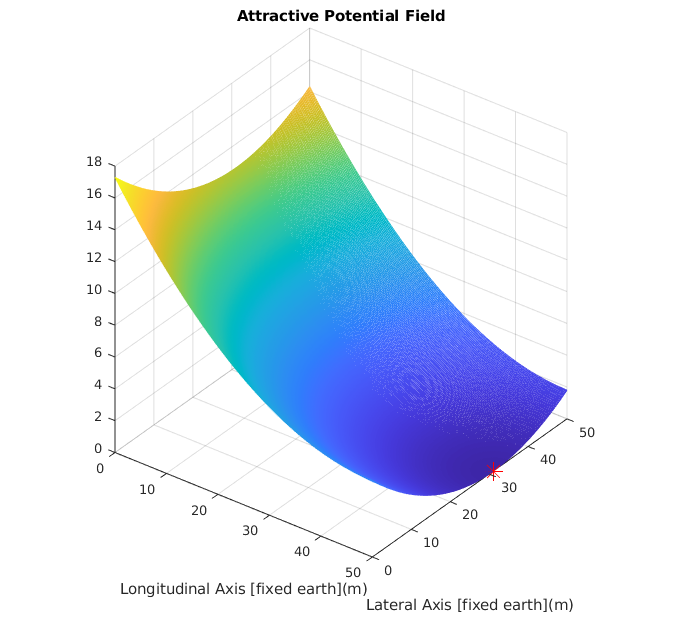
\includegraphics[scale=0.45]{presentation/img/u_att.png}
    \caption{Attractive Potential Field}
    \label{fig:u_att}
\end{figure}


The second component of the universal potential is the repulsive potential which results from superimposing 
the repulsive potential of each obstacle. The repulsive potential of an obstacle has it's peak at the obstacle and reduces as the 
distance from the obstacle increases. It can be expressed as:

$$
U_{R}(\vec{X_{r}}, \vec{X_{o}}):= \frac{1}{2} K_{rep} \left( \frac{1}{\begin{Vmatrix}\vec{X_{r}} - \vec{X_{o}}\end{Vmatrix}} 
    - \frac{1}{\rho_{0}} \right)
$$

\noindent
$K_{rep}$ is a constant
$\rho_{0}$ is a constant that dictates the maximum distance from which the influence of an obstacle can be felt.

\noindent
A suitable selection according to kinetic theory is $\rho_{0} \geq V_{MAX}/2 A_{MAX}$ where $V_{MAX}$ is the 
maximum speed of the AMR and $A_{MAX}$ is the maximum decceleration of the AMR \cite{rostami1}.

Figure \ref{fig:u_uni_plot} shows the universal potential obtained by fusing the attractive potential from Figure \ref{fig:u_att} with repulsive 
potentials obtained from circular obstacles of radius $1m$ at coordinates (14.87, 33.28), (10, 8), (26, 12), (19, 19), and (34, 23) 
with $K_{rep}= 10$.


\begin{figure}
    \centering
    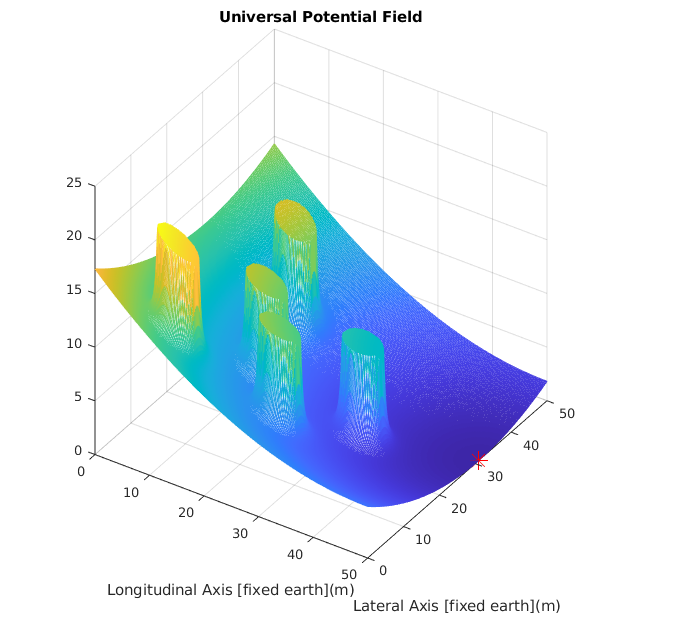
\includegraphics[scale=0.45]{presentation/img/u_uni_plot.png}
    \caption{Universal Potential Field}
    \label{fig:u_uni_plot}
\end{figure}


After setting up the universal potential, a simple gradient descent along this potential yields a "force" that guides the AMR towards the goal position 
while deflecting it away from the obstacles. This force can be interpreted as the velocity vector of the AMR along the planned path, 
it can be expressed as: 

$$F:= F_{A} + F_{R}$$
\noindent
where $F_{A}$ is the attractive force which is given by:
$$F_{A}(\vec{X_{r}}, \vec{X_{o}}):= -grad(U_{A})$$
$$F_{A}(\vec{X_{r}}, \vec{X_{o}})= -K_{att} \left(\vec{X_{r}} - \vec{X_{g}}\right)$$
\noindent
and $F_{R}$ is the repulsive force which is given by:
$$F_{R}(\vec{X_{r}}, \vec{X_{o}}):= \sum_{ \vec{X_{o}} \in \Omega}{-grad(U_{R})} $$
$$-grad(U_{R})= \frac{K_{rep}}{\rho^{3}} 
        \left( \frac{1}{\rho} - \frac{1}{\rho_{0}} \right) 
        \left(\vec{X_{r}} - \vec{X_{o}}\right) $$
\noindent
with $\rho= \begin{Vmatrix}\vec{X_{r}} - \vec{X_{o}}\end{Vmatrix}$ and $\Omega$ is a set of all obstacle coordinates.
 
Building upon the universal potential depicted in Figure \ref{fig:u_uni_plot}, Figure \ref{fig:path} shows the resulting collision-free path from the AMR's initial position (0, 0) to the goal position (50, 30).

\begin{figure}
    \centering
    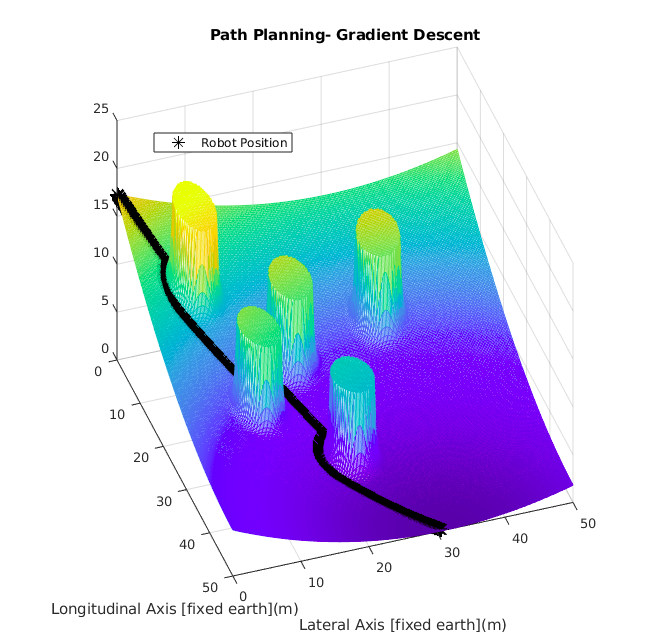
\includegraphics[scale=1.2]{presentation/img/path.png}
    \caption{Gradient descent along Universal Potential Field}
    \label{fig:path}
\end{figure}




\subsection{Trajectory Generation}

A planned-path can be transformed into a trajectory by time-parametizing it \cite{roesmann1}. 
Following from our earlier assumption of the Autonomous Mobile Robot (AMR) having a constant velocity of $1m/s$, 
we can generate a trajectory from our planned path by simulating forward in time along the planned path with a velocity 
vector of magnitude $1m/s$.

\noindent
Figures \ref{fig:traj_lat} and \ref{fig:traj_lon} show the trajectory information for the path illustrated in \ref{fig:path} simulated with a 
sampling time of 0.1 seconds.


\begin{figure}
    \centering
    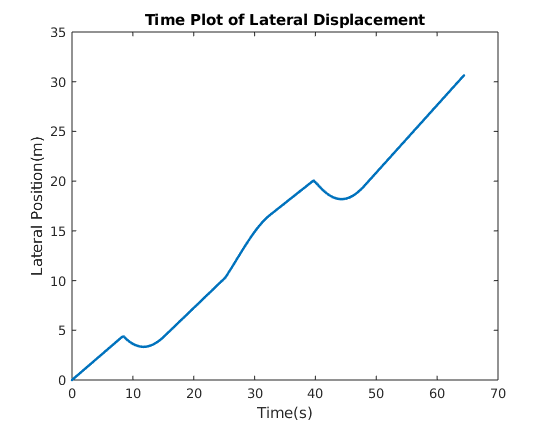
\includegraphics[scale=.45]{presentation/img/traj_lat.png}
    \caption{Trajectory- Lateral Displacement}
    \label{fig:traj_lat}
\end{figure}

\begin{figure}
    \centering
    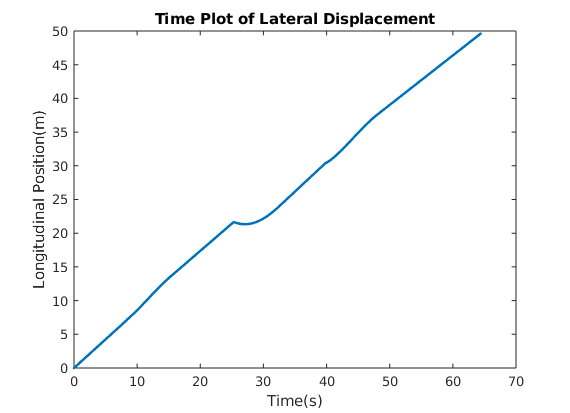
\includegraphics[scale=.45]{presentation/img/traj_lon.png}
    \caption{Trajectory- Longitudinal Displacement}
    \label{fig:traj_lon}
\end{figure}

%===============================================================================================================%
% MPC Controller Design
\section{Mathematical Model for Path Tracking Problem}

The mathematical model used for model predictive controller design is described in this section. Since the success of any controller design is highly 
dependent on the accuracy of the plant model employed, correct modelling of the Autonomous Mobile Robot (AMR) is necessary. While the dynamics of the 
AMR are nonlinear, MPC allows us to base our design on a linearized model and still get satisfactory results. For the path tracking problem considered 
in this paper, the following simplifying assumptions are made:
\begin{itemize}
    \item The AMR is a front wheel controller vehicle with a single front wheel and two real wheels.
    \item Motion is only in the X-Y plane, rolling and pitching motions are ignored.
    \item Model parameters are constant.
    \item The AMR is operating in an indoor environment with a smooth and flat surface such that gravitational and aerodynamic side forces can be ignored.
    \item Constant longitudinal velocity with perfect tracking along the longitudinal axis.
\end{itemize}

\subsection{Dynamic Model for Lateral Path Tracking}
With the above assumptions, and also by lumping the two rear wheel into a single wheel, the linear two degree of freedom bicycle model of a 
conventional vehicle can be employed.

\noindent
Considering Newton's law of conservation of momentum along the lateral-axis, we have:

$$F_{yf} + F_{yr}= \dot{u} + v\dot{\psi}$$
$$l_f F_{yf} - l_r F_{yr}= I_{zz} \dot(\psi) $$

\noindent
Front tyre lateral force
$$
F_{xf}cos(\delta) + F_{xr}= m(\dot{u} - \dot{\psi}v)
$$
Rear tyre lateral force (2 rear tyres)
$$
aF_{xf}cos(\delta) - bF_{xr}= I_{zz}\dot{r}
$$

\noindent
The slip angles are given as:
\\
Front tyre slip angle
$$
\gamma_{f}= atan\left(\frac{u+a\dot{\psi}}{v}\right)- \delta
$$
Rear tyre slip angle
$$
\gamma_{r}= atan\left(\frac{u-b\dot{\psi}}{v}\right)
$$

\noindent
The lateral tire forces can be expressed as:
$$
F_{xf}= C_{f}\gamma_{f}
$$
$$
F_{xr}= 2C_{r}\gamma_{r}
$$

\noindent
The sideslip angle, $\beta= atan\left(\frac{u}{v}\right)$
\\

\noindent
With small angles approximations,

Sideslip angle, 
$$\beta= \frac{u}{v}$$

Front tyre angle, 
$$\gamma_{f}= \frac{u+a\dot{\psi}}{v}- \delta= \beta + \frac{a\dot{\psi}}{v}+ \delta$$

Rear tyre angle, 
$$\gamma_{r}= \frac{u-b\dot{\psi}}{v}= \beta- \frac{b\dot{\psi}}{v}$$


\noindent
The equations of motion then yeild the following differential equations:

\footnotesize 
$$
\dot{\beta}= -\frac{\beta}{mv}\left( C_{f} + 2C_{f} \right) + r \left[\frac{1}{mv^{2}} \left(2bC_{r} 
    - aC_{f}\right)\right] + \delta \frac{C_{f}}{mv}  
$$

$$
\dot{r}= -\frac{\beta}{I_{zz}}\left(aC_{f} - 2bC_{r}\right) - r \left[\frac{1}{I_{zz}v} 
    \left(a^{2}C_{f} + 2b^{2}C_{r}\right) \right] + \delta \frac{aC_{f}}{I_{zz}} 
$$
\\

\normalsize
\noindent
By selecting the state variables:
\begin{itemize}
    \item Lateral displacement of CoM, $x_{c}$
    \item Side-slip angle, $\beta$
    \item Yaw angle, $\psi$
    \item Yaw velocity, $r$
\end{itemize}

\footnotesize
$$
\begin{bmatrix}
    \dot{x_{c}}
    \\
    \dot{\beta}
    \\
    \dot{\psi}
    \\  
    \dot{r}
\end{bmatrix}=
\begin{bmatrix}
    0 & v & v & 0 \\ 
    0 & -\frac{C_{f}+2C_{r}}{mv} & 0 & \frac{2bC_{r} - aC_{f}}{mv^{2}} -1 \\ 
    0 & 0 & 0 & 1 \\ 
    0 & \frac{2bC_{r} - aC_{f}}{I_{zz}} & 0 & -\frac{\left(2b^{2}C_{r} + a^{2}C_{f}\right)}{I_{zz}v} 
\end{bmatrix}
\begin{bmatrix}
    x_{c}
    \\
    \beta
    \\
    \psi
    \\  
    r
\end{bmatrix}+
\begin{bmatrix}
    0
    \\
    \frac{C_{f}}{mv}
    \\
    0
    \\  
    \frac{aC_{f}}{I_{zz}}
\end{bmatrix} \delta$$
\\

\normalsize
\noindent
SISO Model output:
\footnotesize
$$
x_{c}=
\begin{bmatrix}
    1&0&0&0
\end{bmatrix}
\begin{bmatrix}
    x_{c}
    \\
    \beta
    \\
    \psi
    \\  
    r
\end{bmatrix}
$$
\\

\normalsize
\noindent
SIMO Model output:
\footnotesize
$$ 
\begin{bmatrix}
    x_{c} 
    \\
    \psi   
\end{bmatrix}=
\begin{bmatrix}
    1&0&0&0
    \\
    0&0&1&0
\end{bmatrix}
\begin{bmatrix}
    x_{c}
    \\
    \beta
    \\
    \psi
    \\  
    r
\end{bmatrix}
$$

\normalsize

\bibliographystyle{plain}
\bibliography{references} 

\end{document}
